\documentclass[a5paper, 10pt]{tekst}

\usepackage{titlesec}

\begin{document}
	\thispagestyle{empty}
	\onehalfspacing
	\titleformat*{\section}{\sffamily\bfseries}
	\sffamily
	
	\begin{center}
		\Huge \f{地震}{じしん}が\f{起}{お}こったら
	\end{center}
	\vspace{2em}
	
	{\Large\sloppy
		\section{\f{建物}{たてもの}の中にいるとき}
		\begin{figure}[h]
			\centering
			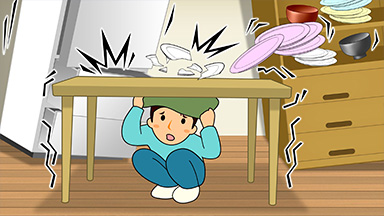
\includegraphics[width=0.5\linewidth]{figures/2017_earthquake1.jpg}		
		\end{figure}
		\p{\f{地震}{じしん}が}\p{\f{起}{お}こったら、}\p{テーブルの}\p{下などに}\p{入って、}\p{\f{揺}{ゆ}れが}\p{\f{止}{と}まるまで}\p{\f{待}{ま}ちましょう。}\p{上から}\p{\f{物}{もの}が}\p{\f{落}{お}ちて}\p{きたり、}\p{\f{本棚}{ほんだな}などの}\p{\f{家具}{かぐ}が}\p{\f{倒}{たお}れたり}\p{して}\p{\f{危険}{きけん}だからです。}\p{ストーブや}\p{ガスの}\p{火は、}\p{\f{揺}{ゆ}れが}\p{\f{止}{と}まってから}\p{\f{消}{け}して}\p{ください。}\p{\f{揺}{ゆ}れて}\p{いる}\p{ときに}\p{火を}\p{\f{消}{け}そうと}\p{すると、}\p{やけどを}\p{する}\p{ことが}\p{あります。}
		
		\section{外に\f{逃}{に}げるとき}
		\begin{figure}[h]
			\centering
			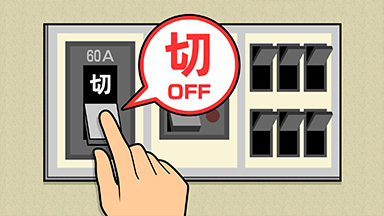
\includegraphics[width=0.5\linewidth]{figures/2017_earthquake2.jpg}		
		\end{figure}
		\p{ブレーカーの}\p{スイッチを}\p{「\f{切}{き}る}\p{(\f{off}{おふ})」に}\p{して}\p{\f{電気}{でんき}を}\p{\f{切}{き}ってから、}\p{外に}\p{出て}\p{ください。}\p{\f{大}{おお}きな}\p{\f{地震}{じしん}では}\p{「\f{停電}{ていでん}」に}\p{なって}\p{\f{電気}{でんき}が}\p{\f{止}{と}まる}\p{ことが}\p{あります。}\p{その}\p{あと}\p{\f{電気}{でんき}が}\p{また}\p{\f{流}{なが}れた}\p{ときに、}\p{ストーブなどが}\p{\f{自動}{じどう}で}\p{ついて、}\p{\f{火事}{かじ}に}\p{なる}\p{ことが}\p{あるからです。}
		
		\section{外にいるとき}
		\begin{figure}[h]
			\centering
			
\includegraphics[width=0.5\linewidth]{figures/2017_earthquake3.jpg}		
		\end{figure}
		\p{ビルの}\p{\f{近}{ちか}くは、}\p{\f{窓}{まど}}\p{ガラスや}\p{\f{看板}{かんばん}などが}\p{\f{落}{お}ちて}\p{くる}\p{ことが}\p{あります。}\p{かばんなどで}\p{\f{頭}{あたま}を}\p{\f{守}{まも}りながら、}\p{\f{安全}{あんぜん}な}\p{\f{場所}{ばしょ}に}\p{\f{逃}{に}げて}\p{ください。}
		
		\begin{figure}[h]
			\centering
			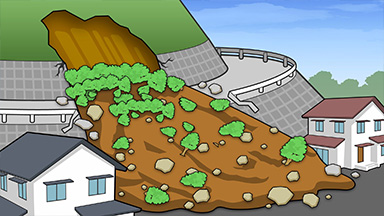
\includegraphics[width=0.5\linewidth]{figures/2017_earthquake4.jpg}		
		\end{figure}
		
		\p{ブロックの}\p{\f{塀}{へい}や}\p{\f{自動}{じどう}}\p{\f{販売}{はんばい}}\p{\f{機}{き}など}\p{\f{倒}{たお}れやすい}\p{\f{物}{もの}の}\p{\f{近}{ちか}くも}\p{\f{危険}{きけん}です。}\p{山や}\p{\f{崖}{がけ}などは}\p{\f{崩}{くず}れて}\p{\f{危険}{きけん}ですから、}\p{\f{遠}{とお}くに}\p{\f{逃}{に}げて}\p{ください。}
		
		\section{車を\f{運転}{うんてん}しているとき}
		\p{車を}\p{ゆっくり}\p{\f{道}{みち}の}\p{\f{左側}{ひだりがわ}に}\p{\f{止}{と}めて、}\p{エンジンを}\p{\f{切}{き}ります。}\p{車を}\p{\f{道}{みち}に}\p{\f{置}{お}いて}\p{\f{逃}{に}げる}\p{\f{場合}{ばあい}は、}\p{ドアに}\p{\f{鍵}{かぎ}を}\p{かけないで、}\p{車に}\p{\f{鍵}{かぎ}を}\p{\f{付}{つ}けた}\p{ままに}\p{して}\p{おきましょう。}\p{\f{救急}{きゅうきゅう}\f{車}{しゃ}や}\p{\f{警察}{けいさつ}などの}\p{車が}\p{\f{通}{とお}る}\p{ときに、}\p{\f{動}{うご}かす}\p{ことが}\p{あるからです。}
	}
	
	\clearpage
	\titleformat*{\section}{\rmfamily\bfseries}
	\rmfamily
	
	\section*{Vokabular}\noindent
	\begin{multicols}{2}[{\centering\textbf{Bitno}}]
		\dictentry{起こる \strut}{おこる}{\item dogoditi se}{glagol {\upshape (五)}}
		\dictentry{建物 \strut}{たてもの}{\item građevina}{imenica}
		\dictentry{止まる \strut}{とまる}{\item stati}{glagol {\upshape (五)}}
		\dictentry{待つ \strut}{まつ}{\item čekati}{glagol {\upshape (五)}}
		\dictentry{家具 \strut}{かぐ}{\item namještaj}{imenica}
		\dictentry{逃げる \strut}{にげる}{\item pobjeći}{glagol {\upshape (一)}}
		\dictentry{危険 \strut}{きけん}{\item opasnost}{imenica, no-pridjev}
		\dictentry{塀 \strut}{へい}{\item zid}{imenica}
		\dictentry{場合 \strut}{ばあい}{\item situacija, slučaj}{priložna imenica}
		\dictentry{通る \strut}{とおる}{\item proći}{glagol {\upshape (五)}}
		\dictentry{動かす \strut}{うごかす}{\item pomaknuti}{glagol {\upshape (五)}}
	\end{multicols}
	\begin{multicols}{2}[{\centering\textbf{Ostalo}}]
		\dictentry{地震 \strut}{じしん}{\item potres}{imenica}
		\dictentry{中 \strut}{なか}{\item unutar, sredina}{imenica}
		\dictentry{下 \strut}{した}{\item ispod, dolje}{imenica}
		\dictentry{入る \strut}{はいる}{\item ući}{glagol {\upshape (五)}}
		\dictentry{揺れ \strut}{ゆれ}{\item trešnja}{imenica}
		\dictentry{上 \strut}{うえ}{\item gore, iznad}{imenica}
		\dictentry{物 \strut}{もの}{\item stvar}{imenica}
		\dictentry{落ちる \strut}{おちる}{\item pasti}{glagol {\upshape (一)}}
		\dictentry{本棚 \strut}{ほんだな}{\item biblioteka}{imenica}
		\dictentry{倒れる \strut}{たおれる}{\item opasti}{glagol {\upshape (一)}}
		\dictentry{火 \strut}{ひ}{\item vatra}{imenica }
		\dictentry{消す \strut}{けす}{\item ugasiti}{glagol {\upshape (五)}}
		\dictentry{外 \strut}{そと}{\item vani}{imenica}
		\dictentry{切る \strut}{きる}{\item rezati, ugasiti}{glagol {\upshape (五)}}
		\dictentry{電気 \strut}{でんき}{\item struja}{imenica}
		\dictentry{出る \strut}{でる}{\item izaći}{glagol {\upshape (一)}}
		\dictentry{大きい \strut}{おおきい}{\item velik}{i-pridjev}
		\dictentry{停電 \strut}{ていでん}{\item nestanak struje}{imenica, suru-glagol {\upshape (一)}}
		\dictentry{流れる \strut}{ながれる}{\item teći}{glagol {\upshape (一)}}
		\dictentry{自動 \strut}{じどう}{\item automatski}{no-pridjev, imenica}
		\dictentry{火事 \strut}{かじ}{\item požar}{imenica}
		\dictentry{近い \strut}{ちかい}{\item blizu}{i-pridjev}
		\dictentry{窓 \strut}{まど}{\item prozor}{imenica}
		\dictentry{看板 \strut}{かんばん}{\item natpis, pano, reklama}{imenica}
		\dictentry{頭 \strut}{あたま}{\item glava}{imenica}
		\dictentry{守る \strut}{まもる}{\item zaštititi}{glagol {\upshape (五)}}
		\dictentry{安全 \strut}{あんぜん}{\item sigurno(-st)}{imenica, na-pridjev}
		\dictentry{場所 \strut}{ばしょ}{\item mjesto}{imenica}
		\dictentry{自動販売機 \strut}{じどうはんばいき}{\item automat}{imenica}
		\dictentry{山 \strut}{やま}{\item planina}{imenica, brojač}
		\dictentry{崖 \strut}{がけ}{\item litica}{imenica}
		\dictentry{崩れる \strut}{くずれる}{\item srušiti se}{glagol {\upshape (一)}}
		\dictentry{遠い \strut}{とおい}{\item dalek}{i-pridjev}
		\dictentry{車 \strut}{くるま}{\item automobil}{imenica}
		\dictentry{運転 \strut}{うんてん}{\item vožnja, voziti}{imenica, no-pridjev, suru glagol}
		\dictentry{道 \strut}{みち}{\item put, cesta}{imenica}
		\dictentry{左側 \strut}{ひだりがわ}{\item lijeva strana}{imenica, no-pridjev}
		\dictentry{置く \strut}{おく}{\item ostaviti}{glagol {\upshape (五)}}
		\dictentry{鍵を付ける \strut}{かぎをかける}{\item zaključati}{izraz}
		\dictentry{救急車 \strut}{きゅうきゅうしゃ}{\item hitna pomoć}{imenica}
		\dictentry{警察 \strut}{けいさつ}{\item policija}{imenica}
	\end{multicols}
	
	\section*{Zadaci}
	\begin{enumerate} 
		\item Sažmite tekst u najviše dvije rečenice.
		\item Razgovarajte o tekstu.
	\end{enumerate}
	
	\section*{Domaća zadaća}
	\begin{enumerate}
		\item Napišite kratku priču ili par rečenica koristeći barem 5 riječi iz teksta. Rečenice ili tekst ne moraju nužno biti vezane uz samu vijest. 
		\item Odgovorite na pitanja:
		\begin{enumerate}[label=(\roman*)]
			\item \p{\f{地震}{じしん}の}\p{時に}\p{\f{建物}{たてもの}の}\p{中に}\p{いると}\p{何を}\p{しなければ}\p{ならないのですか?}
			\item \p{大きな}\p{\f{地震}{じしん}の}\p{時に}\p{\f{何}{なん}が}\p{\f{起}{お}こるんですか?}
			\item \p{外に}\p{いると}\p{\f{何}{なん}に}\p{\f{注意}{ちゅうい}}\p{しなければ}\p{なりませんか?}
			\item \p{何で}\p{車に}\p{\f{鍵}{かぎ}を}\p{\f{付}{つ}けた}\p{ままに}\p{して}\p{おく}\p{ことを}\p{しますか?}
		\end{enumerate}
		
		\item Nadopunite sljedeće rečenice riječima iz vokabulara:
		\begin{enumerate}[label=(\roman*)]
			\item \p{\ansline{}な}\p{ものが}\p{\ansline{}と、}\p{すぐに}\p{\f{助}{たす}けを}\p{\f{求}{もと}めて}\p{ください。}
			\item \p{\f{古}{ふる}い}\p{\ansline{}の}\p{中に}\p{\ansline{}を}\p{\f{見}{み}つけたら}\p{\f{自分}{じぶん}の}\p{\f{家}{いえ}に}\p{\f{持}{も}って}\p{\f{帰}{かえ}る}\p{ことは}\p{だめです。}
			\item \p{\f{救急}{きゅうきゅう}\f{車}{しゃ}が}\p{\ansline{}まで}\p{けが\f{人}{にん}の}\p{そばから}\p{\f{離}{はな}れてわ}\p{いけません。}
			\item \p{\f{花子}{はなご}ちゃんは}\p{ライオンから}\p{\ansline{}}\p{\f{夢}{ゆめ}を}\p{したから}\p{今は}\p{\f{武}{たけし}くんの}\p{\f{家}{いえ}の}\p{前で}\p{\f{彼}{かれ}に}\p{\f{夢}{ゆめ}の}\p{ことを}\p{話したいから}\p{\ansline{}。}
			\item \p{\f{鈴木}{すずき}さんは}\p{\ansline{}を}\p{\ansline{}と}\p{して}\p{いる。}
			\item \p{\f{弾}{たま}が}\p{ヘルメットを}\p{\ansline{}}\p{\ansline{}}\p{\f{武}{たけし}くんは}\p{\f{死}{し}ぬだろう。}
		\end{enumerate}
	\end{enumerate}
\end{document}